\begin{figure}[t!]
  \centering
  \begin{subfigure}{0.5\linewidth}
    \centering
    \footnotesize
    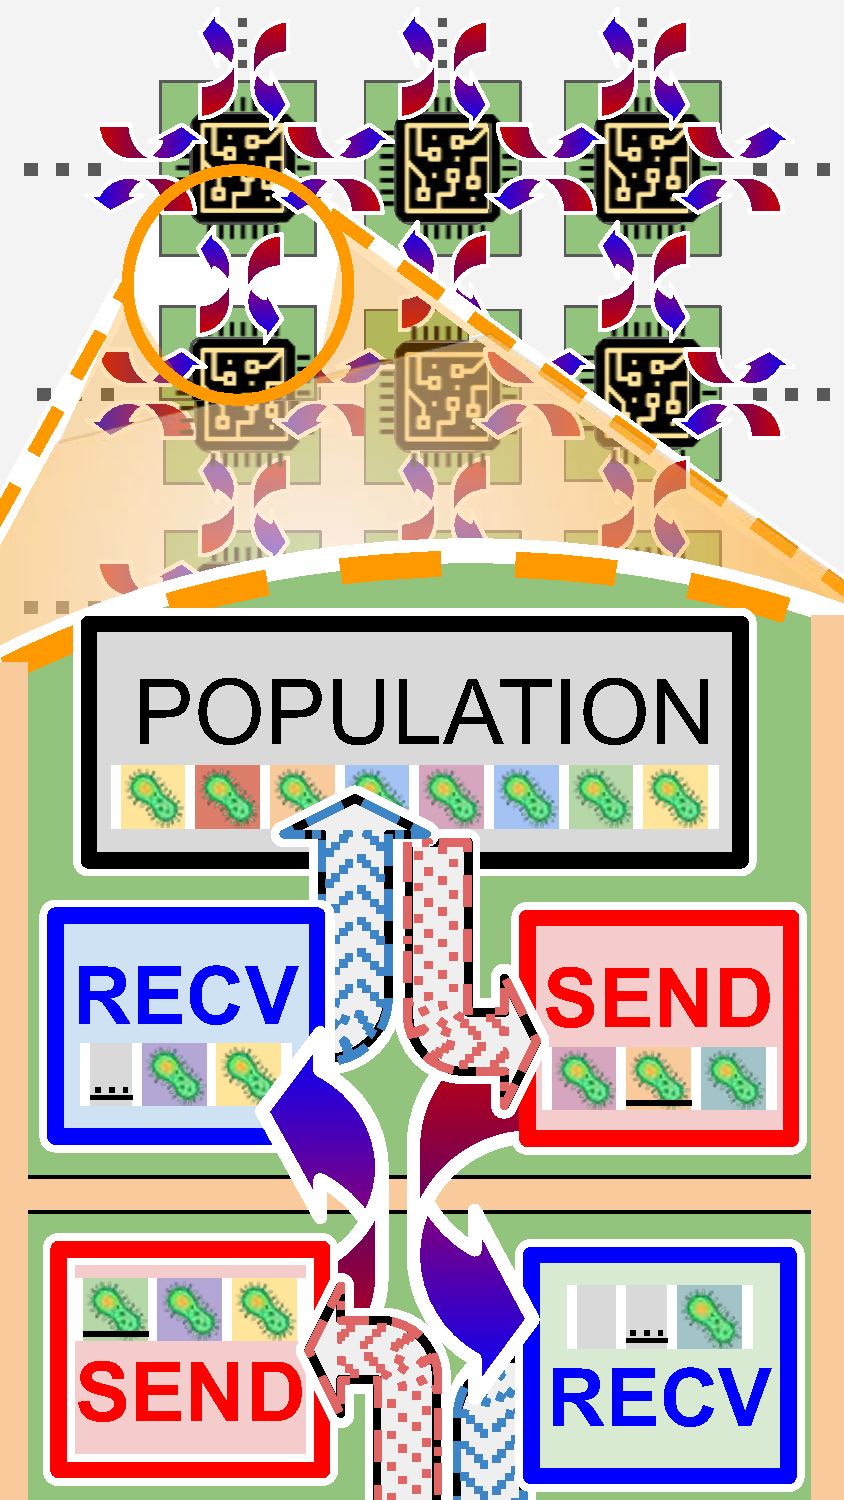
\includegraphics[width=0.8\linewidth]{img/dataflow-schematic}
    \vspace{-0.05in}
    \caption{data flow between PEs}
  \end{subfigure}%
  \begin{subfigure}{0.5\linewidth}
    \footnotesize
    \centering
    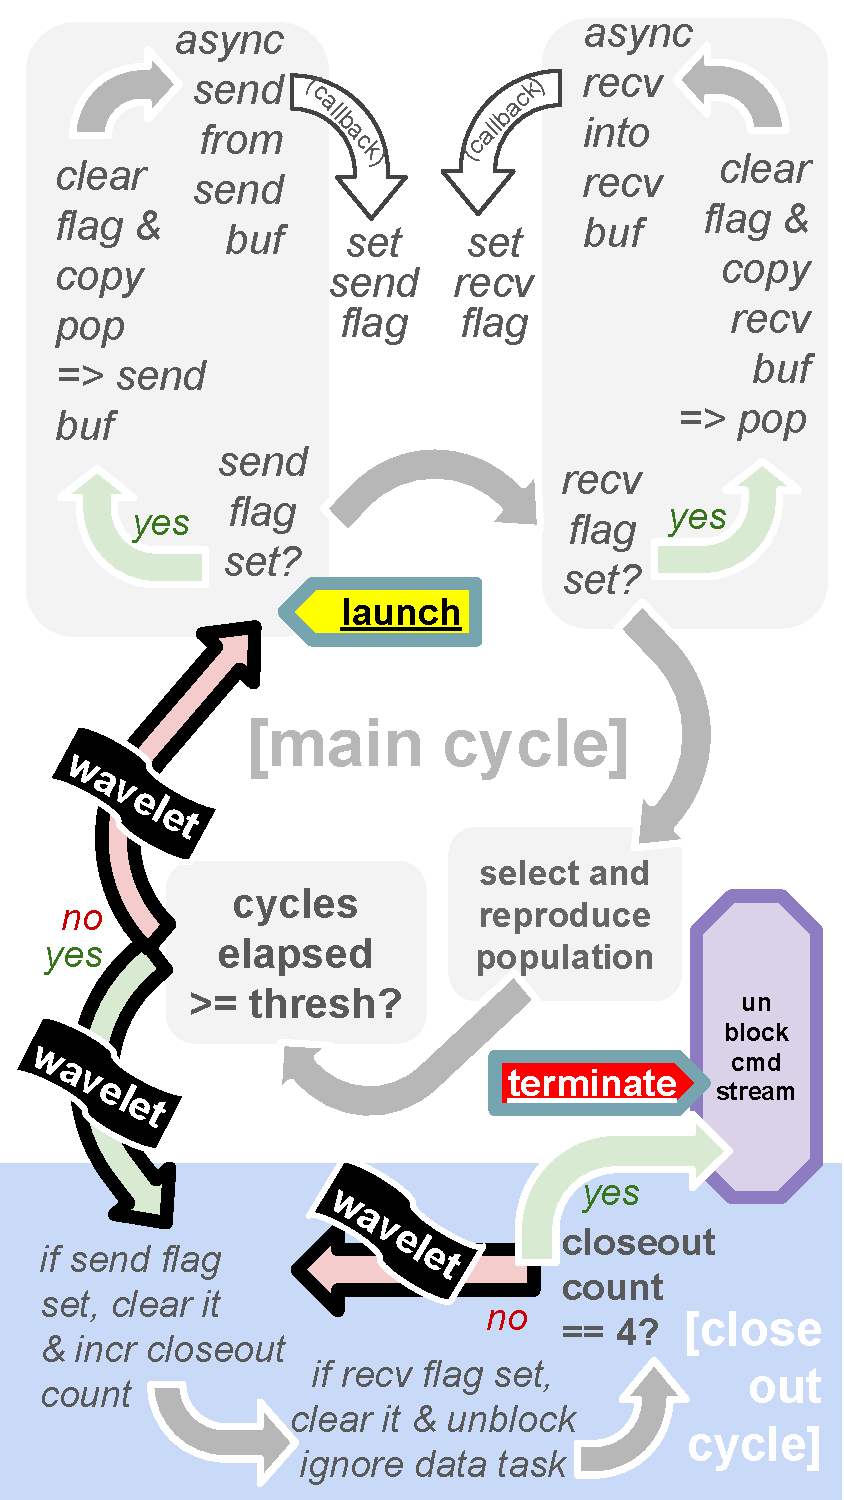
\includegraphics[width=0.8\linewidth]{img/controlflow-schematic}%
    \vspace{-0.05in}
    \caption{control flow within PE}
  \end{subfigure}
  \vspace{-0.25in}
  \caption{%
  \textbf{Island model GA implementation for WSE.}
  \footnotesize
  Neighboring PEs exchange agents (🦠) via asynchronous send/receive operations from dedicated buffers (``migration''), with on-completion callbacks setting ``ready'' flags to copy between main population and ready buffer.
  }
  \label{fig:async-ga-schematic}
  \vspace{-0.2in}
\end{figure}
